\draft Symmetry and active modes.

\begin{parts}
	\part
	\begin{subparts}
		\subpart IR spectroscopy involves shining an infrared beam through a sample and measuring the absorption.
		The absorption corresponds to the energy taken to excite a vibrational mode via the electric dipole interaction.
		Since the electric dipole is involved, the mode must possess similar symmetry to a component of polarisation.
		
		\subpart
		\begin{figure}[H]
			\centering
			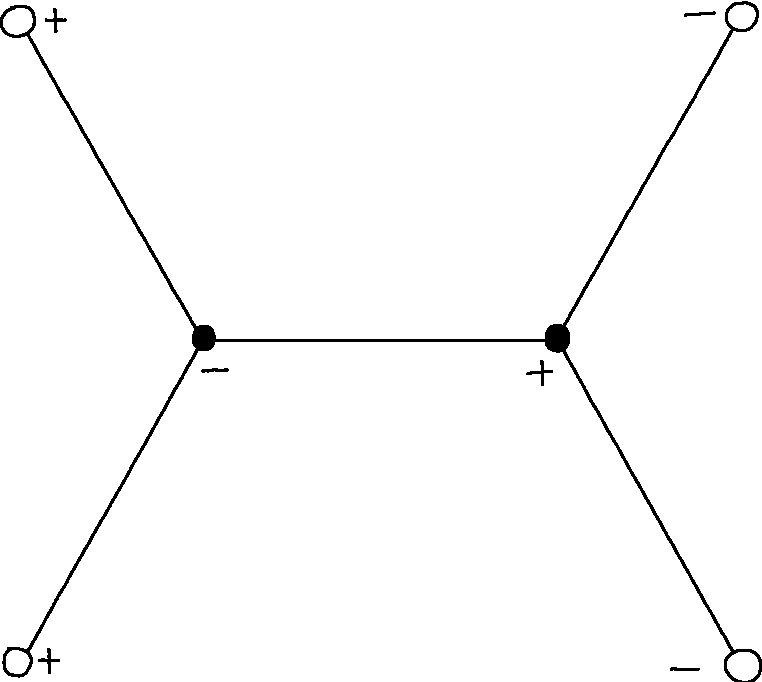
\includegraphics[width=.25\linewidth]{q1-v1}
			\hspace{.05\linewidth}
			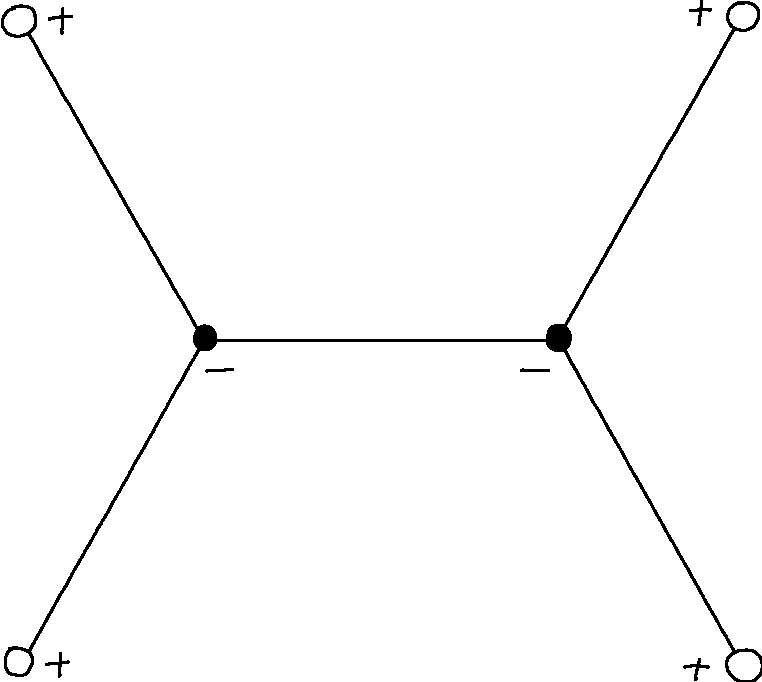
\includegraphics[width=.25\linewidth]{q1-v2}
			\hspace{.05\linewidth}
			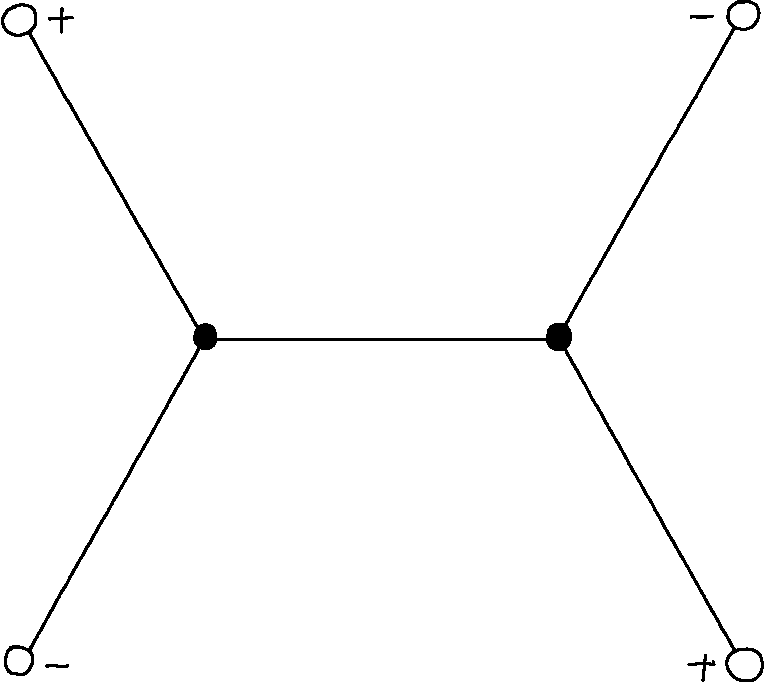
\includegraphics[width=.25\linewidth]{q1-v3}
		\end{figure}
		For $V_1$:
		\begin{align*}
			m_x:\; -1 \qquad m_y:\; +1 \qquad m_z:\; -1
		\end{align*}
		
		For $V_2$:
		\begin{align*}
			m_x:\; +1 \qquad m_y:\; +1 \qquad m_z:\; -1
		\end{align*}
		
		For $V_3$:
		\begin{align*}
			m_x:\; -1 \qquad m_y:\; -1 \qquad m_z:\; -1
		\end{align*}
		
		Character table for polarisation:
		
		\begin{center}
			\begin{tabular}{|c|c|c|c|}
				& $m_x$ & $m_y$ & $m_z$ \\
				$p_x$ & $-1$ & $+1$ & $+1$ \\
				$p_y$ & $+1$ & $-1$ & $+1$ \\
				$p_z$ & $+1$ & $+1$ & $-1$
			\end{tabular}
		\end{center}
		
		So only $V_2$ is IR active in $p_z$.
		
		\subpart
		\begin{align*}
			\textnormal{\# of modes} &= 3 \times 6 \mtext{atoms} \\
			&= 18 \\
			&= \underbracket{\textnormal{\# translational}}_{3} + \underbracket{\textnormal{\# rotational}}_{3} + \textnormal{\# vibrational}
		\end{align*}
		
		So we have 9 additional vibration modes.
	\end{subparts}
	
	\part \# of phonon modes: \# of particles in a primitive UC = 4
	
	There are 2 acoustic modes and 2 optic modes.
	
	\part
	\begin{subparts}
		\subpart From the diagram,
		\begin{align*}
			\mathbf{a}_r &= \mathbf{a}_p + \mathbf{b}_p \\
			\mathbf{b}_r &= \mathbf{b}_p - \mathbf{a}_p \\
			\Rightarrow \mathbf{b}_p &= \frac{\mathbf{a}_r + \mathbf{b}_r}{2} \\
			\mathbf{a}_p &= \frac{\mathbf{a}_r - \mathbf{b}_r}{2}
		\end{align*}
		
		\subpart Definition of reciprocal basis:
		\begin{equation*}
			\mathbf{a}_p^* = 2\pi \frac{\mathbf{b}_p \times \mathbf{z}}{\mathbf{a}_p \cdot \rbracket{\mathbf{b}_p \times \mathbf{z}}}
		\end{equation*}
		
		\begin{align*}
			\Rightarrow \mathbf{a}_p^* &= 2\pi \cdot \frac{1}{V} \cdot \frac{1}{2} \rbracket{\underbracket{\mathbf{a}_r \times \mathbf{z}}_{-\mathbf{b}_r^* \cdot 2V/2\pi} + \underbracket{\mathbf{b}_r \times \mathbf{z}}_{\mathbf{a}_r^* \cdot 2V/2\pi}} \mtext{since rectangular lattice has $2\times$area} \\
			&= \rbracket{\mathbf{a}_r^* - \mathbf{b}_r^*} \\
			\mathbf{b}_p^* &= \frac{2\pi}{V} \cdot \frac{1}{2} \rbracket{\underbracket{\mathbf{z} \times \mathbf{a}_r}_{\mathbf{b}_r^* \cdot 2V/2\pi} - \underbracket{\mathbf{z} \times \mathbf{b}_r}_{-\mathbf{a}_r^* \cdot 2V/2\pi}} \\
			&= \mathbf{a}_r* + \mathbf{b}_r^*
		\end{align*}
		
		So Miller indices
		\begin{tabular}{cc}
			& $h_p \mathbf{a}_p^* = h_p \mathbf{a}_r^* - h_p \mathbf{b}_r^*$ \\
			$+)$ & $k_p \mathbf{b}_p^* = k_p \mathbf{a}_r^* + k_p \mathbf{b}_r^*$ \\
			\hline
			& $h_p \mathbf{a}_p^* + k_p \mathbf{b}_p^* = \underbracket{\rbracket{h_p + k_p}}_{h_r} \mathbf{a}_r^* + \underbracket{\rbracket{-h_p + k_p}}_{k_r} \mathbf{b}_r^*$
		\end{tabular}
		
		\begin{equation*}
			\Rightarrow k_p = \frac{h_r + k_r}{2} \qquad h_p = \frac{h_r - k_r}{2}
		\end{equation*}
		
		\subpart \todo $\alpha = \beta = \frac{1}{2}$???
	\end{subparts}
	
	\part
	\begin{subparts}
		\subpart From c we have $h_p = \rbracket{h_r - k_r}/2$ and $k_p = \rbracket{h_r + k_r}/2$:
		\begin{align*}
			\Rightarrow P_1 &= \rbracket{\frac{1-0}{2}, \frac{1+0}{2}} = \rbracket{\frac{1}{2}, \frac{1}{2}} \\
			P_2 &= \rbracket{\frac{0-0}{2}, \frac{0+0}{2}} = \rbracket{0, 0}
		\end{align*}
		in the primitive lattice.
		
		\subpart For a phonon to be measurable by IR spectroscopy, it needs to be excited by the IR beam, thus the probable mode must have low momentum (i.e. near BZ boundary) due to the light having large dispersion gradient.
		\begin{figure}[H]
			\centering
			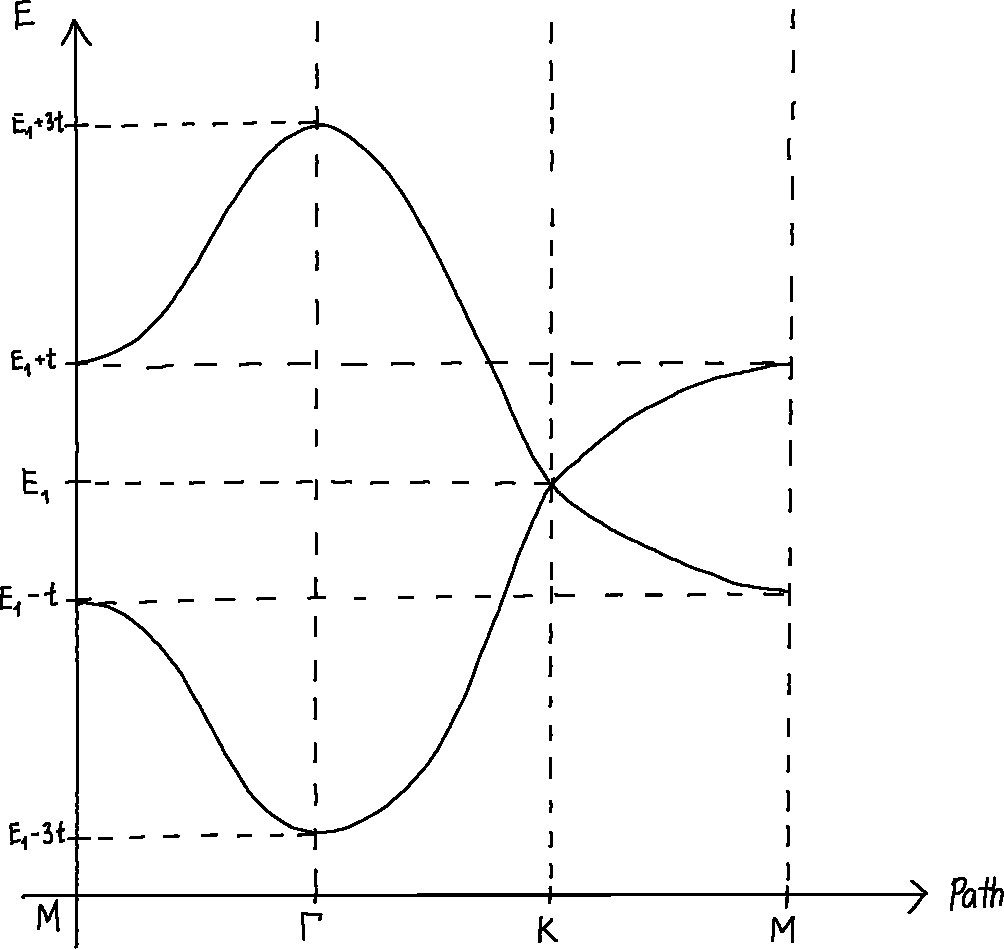
\includegraphics[width=.6\linewidth]{q1-dispersion}
		\end{figure}
		
		\subpart \todo $P_2$ is IR active due to the null wavevector?
	\end{subparts}
\end{parts}